%---------------------------------------------------------------------
% Course 	: Introduction To web sciences
% Professor : Dr.Nelson
% Name   	: Manoj Chandra Kompalli
% Assignment: 7
%---------------------------------------------------------------------
\documentclass[12pt]{article}
%--------------------------------------------------------------------
% packages required
%--------------------------------------------------------------------
\usepackage{graphicx}
\usepackage{listings}
\usepackage{hyperref}
\usepackage{caption}
\usepackage{color}
\usepackage{pdfpages}
\graphicspath{ {images/} }
%--------------------------------------------------------------------
% Start Margins
%--------------------------------------------------------------------
\addtolength{\oddsidemargin}{-.875in}
\addtolength{\evensidemargin}{-.875in}
\addtolength{\textwidth}{1.75in}
\addtolength{\topmargin}{-.885in}
\addtolength{\textheight}{1.95in}
%-------------------------------------------------------------------
% End Margins
%--------------------------------------------------------------------
\definecolor{codegreen}{rgb}{0,0.6,0}
\definecolor{codegray}{rgb}{0.5,0.5,0.5}
\definecolor{codepurple}{rgb}{0.58,0,0.82}
\definecolor{backcolour}{rgb}{0.95,0.95,0.92}
 
\lstdefinestyle{mystyle}{
    backgroundcolor=\color{backcolour},   
    commentstyle=\color{codegreen},
    keywordstyle=\color{magenta},
    numberstyle=\tiny\color{codegray},
    stringstyle=\color{codepurple},
    basicstyle=\footnotesize,
    breakatwhitespace=false,         
    breaklines=true,                 
    captionpos=b,                    
    keepspaces=true,                 
    numbers=left,                    
    numbersep=5pt,                  
    showspaces=false,                
    showstringspaces=false,
    showtabs=false,                  
    tabsize=2
}
 
\lstset{style=mystyle}

\begin{document}

\begin{titlepage}
\title{INTRODUCTION TO WEB SCIENCES:\\*Assignment 7}
\author{Manoj Chandra Kompalli}
\date{31 March 2016}
\maketitle
\end{titlepage}

\tableofcontents
\newpage

\section{Question 1:  }
1.  Find 3 users who are closest to you in terms of age, 
gender, and occupation.  For each of those 3 users:

- what are their top 3 favorite films?
- bottom 3 least favorite films?

Based on the movie values in those 6 tables (3 users X (favorite +
least)), choose a user that you feel is most like you.  Feel 
free to note any outliers (e.g., "I mostly identify with user 123,
except I did not like ``Ghost'' at all").  

This user is the "substitute you".  

\subsection{Approach}
Here my task was to find out a substitute of me.
\begin{itemize} 
 \item I have used the u.user file to collect the user data.
 \item I extracted all the users matching with my age, gender, occupation
 \item I extracted the top 3 from my list
 \item For each user, I stored the itemids and rating from u.data file in a dictionary
 \item I have sorted the dictionary based on the rating
 \item	I have extracted the top three most rated and least rated three items
 \item	I have extracted the movie names for the items using u.items
 \item I have observed that user 33 has two of my favourite movies like Titanic and Tomorrow never dies.
 \item	Therefore, I chose user 33 to be my substitute

\end{itemize}


 \newpage

\subsection{Code Listing}
\subsubsection{substitute.py to generate favorite and least favorite movies }
\lstinputlisting[breaklines=True,language=Python]{../../q1/substitute.py}
\newpage


\subsection{Generated output on shell}
\begin{figure}[ht]
\includegraphics[scale=0.7]{../../q1/output.png}
\centering
\caption{Top and least rated movies and their ratings of user 33}
\label{fig:Top and least rated movies and their ratings of user 33}
\end{figure}


\newpage
\section{Question 2: }
2.  Which 5 users are most correlated to the substitute you? Which
5 users are least correlated (i.e., negative correlation)?


\subsection{Approach}
 Here, I used the recommendations.py file mentioned in the book Programming Collective Intelligence .

\begin{itemize}
\item I have used topMatches() method to extract the users correlated with my substitute user(user 33). 
\item I have stored the results in a dictionary and extracted the top five users from it for the users with most correlation
\item I have extracted the bottom five users from the same dictionary to get the bottom five for the users with least correlation


\end{itemize}

\subsection{Code Listing}
\subsubsection{correlation.py}
\lstinputlisting[breaklines=True,language=Python]{../../q2/correlation.py}
\newpage
\subsection{Output}
\subsubsection{Response showing most and least correlated users to my substitute }
\begin{figure}[ht]
\includegraphics[scale=0.8]{../../q2/output.png}
\centering
\caption{Pearson Coefficients and Correlated users to user 33}
\label{Correlated users to user 33}
\end{figure}
\newpage


\section{Question 3: }
3.  Compute ratings for all the films that the substitute you
have not seen.  Provide a list of the top 5 recommendations for films
that the substitute you should see.  Provide a list of the bottom
5 recommendations (i.e., films the substitute you is almost certain
to hate). 
\subsection{Approach}
 My substitute you has seen and liked a fair bit of movies. Based on this dataset I have to find the most recommended movies and least recommended movies for my substitute.
\begin{itemize} 

\item I used the getRecommendations method from recommendations.py which returned me all the recommended movies for a particular user. 
\item I fetched the movie titles and their respective ratings for all the resulting movie titles
\item The resulting movies are sorted based on their ratings   
\end{itemize}
\subsection{Code Listing}
\subsubsection{recsub.py}
\lstinputlisting[breaklines=True,language=Python]{../../q3/recsub.py}
\newpage
\subsection{Output}
\subsubsection{Top movies along with their ratings}
\begin{figure}[ht]
\includegraphics[scale=0.9]{../../q3/output.png}
\centering
\caption{Recommended movies sorted based on ratings}
\label{Recommended movies sorted based on ratings}
\end{figure}

\section{Question 4: }
4.  Choose your (the real you, not the substitute you) favorite and
least favorite film from the data.  For each film, generate a list
of the top 5 most correlated and bottom 5 least correlated films.
Based on your knowledge of the resulting films, do you agree with
the results?  In other words, do you personally like / dislike
the resulting films?
\subsection{Approach}
My favorite movie is Shawshank Redemption by a long way. Although there are many movies which belong to least favorite movie, I chose Smile like yours. It’s rated 4.2 in IMDB right now. Now, my next job is to get the most correlated movies and least correlated movies for both my favorite and least favorite movies.
\begin{itemize} 
\item To show correlation, again I have used Pearson’s Coefficients.
\item Some of the key functions I used from recommendations.py to extract the data are loadMovieLens which loads the movie lens data, topMatches which sorts the dictionary containing movie items and pearson coefficient. 
\item TopMatches again calls a method ``simpearson'' which finds the preferences and ultimately Pearson score.
\item A Pearson score closer to 1 shows highly correlated movies and score close to -1 shows least correlated movies.
\item I have calculated all twenty scores for my favorite and least favorite films.
\item Unfortunately though I cannot comment on whether I like or dislike the resulting movies because I have hardly watched any of them
\end{itemize}
\subsection{Code Listing}
\subsubsection{myfav.py}
\lstinputlisting[breaklines=True,language=Python]{../../q4/myfav.py}
\newpage
\subsection{Output}
\subsubsection{Response showing Pearson's Coefficient along with correlated movies for Shawshank Redemption and A Smile like yours }
\begin{figure}[ht]
\includegraphics[scale=0.9]{../../q4/output.png}
\centering
\caption{Pearson's Coefficient and movie name}
\label{Pearson's Coefficient and movie name}
\end{figure}
\newpage



\addcontentsline{tableofcontents}{section}{References}





\bibliographystyle{plain}
\bibliography{references}
\cite{*}
\end{document}